\documentclass[french,12pt]{article}
\usepackage[T1]{fontenc}
\usepackage{babel, fontspec, lmodern, etoc, hyperref, geometry, graphicx}
\geometry{
	a4paper,
	left=20mm,
	right=20mm,
	top=20mm,
	bottom=20mm
}
\renewcommand{\familydefault}{\sfdefault}
\setlength{\parindent}{0mm}
\setcounter{tocdepth}{2}
\hypersetup{hidelinks}

% Document begins here
\begin{document}

	% Title page
	\begin{titlepage}
		\begin{center}

			\vspace*{\fill}

			{\Huge
				La Bouée Corsaire
			}\\ [0.5cm]
			{\large
				version 1.4 - \today
			}\\

			\vspace*{\fill}

			{\Large
				Projet réalisé par La Code Académie
			}\\ [0.5cm]
			{\large
				\href{mailto:codeacademie@fondationface.org}{
					codeacademie@fondationface.org
				}
			}\\

			\vspace*{\fill}

			{\Large
				Antoine Le Gonidec
			}

			\vspace*{\fill}

		\end{center}
	\end{titlepage}

	% Table of contents
	\newpage
	\tableofcontents

	% Document history
	\newpage
	\section{Historique du document}
	\begin{description}
		\item [1.0] (23 novembre 2016) première version de travail
		\item [1.1] (2 décembre 2016) mise-à-jour du planning
		\item [1.2] (20 décembre 2016) révision des objectifs de la première version
		\item [1.3] (5 janvier 2017) révision des objectifs de la première version
		\item [1.4] (6 janvier 2017) ajout de diagrammes en annexe
	\end{description}

	% Presentation
	\newpage
	\section{Présentation}
		\paragraph{}
			La Bouée Corsaire est un projet de bourse d’échange de services,
			 valorisant les échanges par un système de décompte d’heures pour se
			 passer totalement d’échanges financiers. Ce projet se présente sous la
			 forme d’une application Web où les personnes inscrites peuvent
			 enregistrer des besoins et des services. Les besoins correspondent aux
			 tâches qu’on souhaite voir réalisées mais pour lesquelles on ne pense pas
			 avoir les compétences ou la motivation, et les services sont des tâches
			 qu’on aime effectuer et qu’on se propose de réaliser pour d’autres
			 personnes. Chaque utilisateur du site a un crédit d’heures qui varie de
			 la façon suivante : lorsque un utilisateur répond au besoin d’un autre,
			 la réserve d’heures du premier est créditée du temps passé à résoudre ce
			 besoin, et celle de celui qui avait fait la demande d’aide est débitée du
			 même nombre d’heures. Pour profiter de l’assistance des utilisateurs du
			 projet il faut donc soi-même proposer ses services.
		\paragraph{}
			Cette application doit pouvoir être utilisée au quotidien indépendamment
			 du type de machine cliente utilisée, une emphase particulière est donc
			 mise sur l’accessibilité et la disponibilité.
		\paragraph{}
			L’objectif à long terme du projet est de proposer ce service à des
			 artisans ou PME, ce qui ajoute une contrainte sur les capacités de mise à
			 l’échelle de l’application qui devra pouvoir gérer un panel très large
			 d’utilisateurs.

	% Features
	\newpage
	\section{Fonctionnalités}
		\etocsetnexttocdepth{3}
		\localtableofcontents

		% Users Accounts
		\newpage
		\subsection{Comptes Utilisateurs}

			L’\hyperlink{utilisateur}{Utilisateur} est au centre de
			 l’\hyperlink{application}{Application}, un soin particulier devra donc
			 être apporté au système de gestion des comptes
			 \hyperlink{utilisateur}{Utilisateurs}.\\
			Une fois connecté, un \hyperlink{utilisateur}{Utilisateur} doit pouvoir
			 définir ses \hyperlink{besoin}{Besoins} ainsi que les
			 \hyperlink{service}{Services} qu’il propose.\\

			Un compte \hyperlink{utilisateur}{Utilisateur} liste les informations
			 suivantes, renseignées lors de la création du compte et modifiables par
			 le propriétaire du compte après création :
			\begin{description}
				\item [Pseudonyme]
					information publique, il sert à identifier
					 l’\hyperlink{utilisateur}{Utilisateur} de manière unique sur
					 l’\hyperlink{application}{Application}
				\item [Nom et Prénom]
					informations privées, elle ne seront divulguées que lors d’échanges
					 personnels entre \hyperlink{utilisateur}{Utilisateurs}
				\item [Adresse physique]
					information privée, seul l’\hyperlink{administrateur}{Administrateur}
					 y aura accès
				\item [Adresse e-mail]
					information privée, seul l’\hyperlink{administrateur}{Administrateur}
					 y aura accès
				\item [Mot de passe]
					information privée, sera stockée après un chiffrement asymétrique
					 (impossible de retrouver le mot de passe à partir de sa version
					 chiffrée)
				\item [Région et Ville]
					informations publiques, permet aux
					 \hyperlink{utilisateur}{Utilisateurs} de trouver des
					 \hyperlink{service}{Services} proches de chez eux
				\item [Téléphone]
					(facultatif) niveau de confidentialité au choix de
					 l’\hyperlink{utilisateur}{Utilisateur}
				\item [\hyperlink{quota}{Quota d’heures disponibles}]
					information privée, ne peut pas être modifié directement par
					 l’\hyperlink{utilisateur}{Utilisateur}, définit le nombre d’heures de
					 \hyperlink{service}{Services} auquel un
					 \hyperlink{utilisateur}{Utilisateur} a droit avant de devoir à son
					 tour rendre un \hyperlink{service}{Service}
				\item [Compte actif]
					modifiable par le propriétaire du compte ou
					 l’\hyperlink{administrateur}{Administrateur}, définit si un compte
					 \hyperlink{utilisateur}{Utilisateur} et ses
					 \hyperlink{besoin}{Besoins} et \hyperlink{service}{Services} associés
					 sont ou non visibles dans l’\hyperlink{application}{Application}
			\end{description}

			Une fonctionnalité de ré-initialisation du mot de passe sera proposée en
			 cas d’oubli par le propriétaire du compte. Une fonction de rappel du mot
			 de passe est techniquement incompatible avec un stockage sécurisé de
			 celui-ci en base de données.

		% Needs and Services
		\newpage
		\subsection{Besoins et Services}
			Un \hyperlink{besoin}{Besoin} représente une demande d’un
			 \hyperlink{utilisateur}{Utilisateur}, un \hyperlink{service}{Service}
			 représente une prestation proposée par un
			 \hyperlink{utilisateur}{Utilisateur}.\\

			La gestion des \hyperlink{service}{Services} n’est pas implémentée dans la
			 première version de l’\hyperlink{application}{Application}.\\

			\hyperlink{besoin}{Besoins} et \hyperlink{service}{Services} contiennent
			 les informations suivantes, renseignées par
			 l’\hyperlink{utilisateur}{Utilisateur} lors de leur création et
			 modifiables par celui-ci :
			\begin{description}
				\item [\hyperlink{utilisateur}{Utilisateur} concerné]
					l’\hyperlink{utilisateur}{Utilisateur} exposant le
					 \hyperlink{besoin}{Besoin} ou proposant le
					 \hyperlink{service}{Service}
				\item [Titre]
					une description succincte du \hyperlink{besoin}{Besoin} (exemple :
					 "Plomberie à rénover") ou du \hyperlink{service}{Service} (exemple :
					 "Cours de guitare")
				\item [\hyperlink{categorie}{Catégorie}]
					(facultatif) le champ d’activité du
					 \hyperlink{besoin}{Besoin}/\hyperlink{service}{Service}
				\item [Description]
					une description détaillée du
					 \hyperlink{besoin}{Besoin}/\hyperlink{service}{Service}
				\item [Niveau d’expertise]
					(facultatif pour les \hyperlink{besoin}{Besoins}) à sélectionner dans
					 une liste (Initié, Avancé, Expert), représente le niveau d’expertise
					 pour la tâche en question de l’\hyperlink{utilisateur}{Utilisateur}
					 proposant le \hyperlink{service}{Service}, ou le niveau d’expertise
					 demandé dans le cas d’un \hyperlink{besoin}{Besoin}
				\item [Lieu]
					(facultatif) le lieu où le
					 \hyperlink{besoin}{Besoin}/\hyperlink{service}{Service} devra être
					 accompli
				\item [Statut]
					indique si le \hyperlink{besoin}{Besoin}/\hyperlink{service}{Service}
					 est en attente d’un \hyperlink{utilisateur}{Utilisateur} intéressé,
					 si une \hyperlink{transaction}{Transaction} est en cours ou acceptée,
					 ou s’il a été effectué.
			\end{description}

			Les \hyperlink{categorie}{Catégories} sont une méthode de classement des
			 \hyperlink{besoin}{Besoins}/\hyperlink{service}{Services} permettant de
			 les trier plus efficacement. Elles sont choisies par
			 l’\hyperlink{utilisateur}{Utilisateur}, mais ne peuvent être créées que
			 par l’\hyperlink{administrateur}{Administrateur}.\\

			La gestion des \hyperlink{categorie}{Catégories} n’est pas implémentée
			 dans la première version de l’\hyperlink{application}{Application}.\\

			Les \hyperlink{categorie}{Catégories} contiennent les informations
			suivantes :
			\begin{description}
				\item [Libellé]
					le nom de la \hyperlink{categorie}{Catégorie}
				\item [\hyperlink{categorie}{Catégorie} parente]
					pour permettre de hiérarchiser les \hyperlink{categorie}{Catégories},
					 on peut définir pour chacune une \hyperlink{categorie}{Catégorie}
					 parente.
			\end{description}

			Il doit être possible pour les \hyperlink{utilisateur}{Utilisateurs} de
			 filtrer les \hyperlink{besoin}{Besoins}/\hyperlink{service}{Services} par
			 différent critères :
			\begin{description}
				\item [\hyperlink{utilisateur}{Utilisateur} concerné]
				\item [Titre]
				\item [\hyperlink{categorie}{Catégorie}]
				\item [Région de l’\hyperlink{utilisateur}{Utilisateur}]
				\item [Région du \hyperlink{besoin}{Besoin}/\hyperlink{service}{Service}]
			\end{description}

		% RSS Feed
		\newpage
		\subsection{Flux RSS}

			Un flux RSS est automatiquement généré à partir des publications de
			 nouveaux \hyperlink{besoin}{Besoins}/\hyperlink{service}{Services}.
			 L’abonnement y est possible facilement (idéalement en un clic).

		% Messaging
		\subsection{Messagerie}

			Un système de \hyperlink{messagerie}{Messagerie} interne à l’application
			 permet aux \hyperlink{utilisateur}{Utilisateurs} d’entrer en contact pour
			 discuter des détails autour d’un
			 \hyperlink{besoin}{Besoin}/\hyperlink{service}{Service}, afin d’aboutir à
			 un accord qui résultera en la mise en place d’une
			 \hyperlink{transaction}{Transaction}.\\

			L’échange de \hyperlink{message}{Messages} se fait via un formulaire
			 contenant les champs suivants :
			\begin{description}
				\item [\hyperlink{besoin}{Besoin}/\hyperlink{service}{Service} concerné]
					(pré-rempli si le formulaire est accédé depuis la page d’un
					 \hyperlink{besoin}{Besoin}/\hyperlink{service}{Service})
				\item [\hyperlink{utilisateur}{Utilisateur} répondant au \hyperlink{besoin}{Besoin}/\hyperlink{service}{Service}]
					(pré-rempli)
				\item [Commentaire]
				\item [Évaluation du temps nécessaire pour le \hyperlink{service}{Service} rendu]
					(facultatif)
				\item [Date définie pour le \hyperlink{service}{Service} rendu]
					(facultatif)
			\end{description}

			Il n’est pas possible pour un \hyperlink{utilisateur}{Utilisateur} de
			 modifier un \hyperlink{message}{Message} envoyé.\\

			Chaque envoi de \hyperlink{message}{Message} résultera en un envoi
			 d’e-mail au \hyperlink{destinataire}{Destinataire}, contenant les
			 informations renseignées dans le formulaire ainsi qu’un lien vers la
			 \hyperlink{discussion}{Discussion}. L’\hyperlink{expediteur}{Expéditeur}
			 peut s’il le souhaite en recevoir une copie.\\

			L’\hyperlink{utilisateur}{Utilisateur} à l’origine du
			 \hyperlink{besoin}{Besoin} peut valider la mise en place d’une
			 \hyperlink{transaction}{Transaction} lorsqu’il est en accord avec les
			 conditions et le temps de réalisation suggérés par celui qui propose le
			 \hyperlink{service}{Service}. Cette validation ne sera possible qu’à
			 partir du moment où une date et une durée horaire ont étés définis.\\

			Tous les \hyperlink{message}{Messages} seront historisés pour permettre
			 une consultation par l’\hyperlink{administrateur}{Administrateur}. Seuls
			 l’\hyperlink{administrateur}{Administrateur},
			 l’\hyperlink{expediteur}{Expéditeur} et le
			 \hyperlink{destinataire}{Destinataire}
			 ont accès à un \hyperlink{message}{Message} donné.\\

			L’\hyperlink{administrateur}{Administrateur} peut désactiver un
			 \hyperlink{message}{Message}, auquel cas il est le seul à y avoir accès.

		% Transactions
		\newpage
		\subsection{Transactions}

			Une \hyperlink{transaction}{Transaction} a lieu lorsqu’un
			 \hyperlink{utilisateur}{Utilisateur} fournit un
			 \hyperlink{service}{Service} à un autre.\\
			Après une phase de discussion entre les
			 \hyperlink{utilisateur}{Utilisateurs} concernés, un rendez-vous est pris
			 et le \hyperlink{service}{Service} est effectué. Suite à la réalisation
			 de celui-ci, et après confirmation de la part de
			 l’\hyperlink{utilisateur}{Utilisateur} qui avait posté le
			 \hyperlink{besoin}{Besoin}, un transfert d’heures entre les
			 \hyperlink{quota}{Quotas} des \hyperlink{utilisateur}{Utilisateurs} est
			 effectué automatiquement. Ce transfert correspond à la durée qui avait
			 été décidé lors de la discussion préalable.\\

			C’est ce système de transfert entre les \hyperlink{quota}{Quotas} qui
			 permet à l’\hyperlink{application}{Application} de fonctionner, en
			 poussant les \hyperlink{utilisateur}{Utilisateurs} à proposer des
			 \hyperlink{service}{Services} qui leur permettront d’augmenter leur
			 \hyperlink{quota}{Quota}, qu’ils pourront ensuite utiliser pour poster
			 des \hyperlink{besoin}{Besoins}.\\

			Toutes les \hyperlink{transaction}{Transactions} ainsi que les discussions
			 associées devront être historisées pour permettre une consultation par
			 l’\hyperlink{administrateur}{Administrateur}. Seuls
			 l’\hyperlink{administrateur}{Administrateur} et les
			 \hyperlink{utilisateur}{Utilisateurs} concernés ont accès à l’historique
			 d’une \hyperlink{transaction}{Transaction} donnée.\\

			En addition aux \hyperlink{transaction}{Transactions} classiques, un
			 \hyperlink{utilisateur}{Utilisateur} peut décider d’effectuer un don
			 d’heures à un autre \hyperlink{utilisateur}{Utilisateur}. Dans ce cas les
			 heures seront transférées entre leurs \hyperlink{quota}{Quotas}
			 respectifs sans contrepartie.

		% E-Mailing
		\subsection{Envoi d’e-mails}

			L’\hyperlink{application}{Application} doit pouvoir envoyer des e-mails à
			 destination d’un \hyperlink{utilisateur}{Utilisateur} donné, ainsi que
			 des e-mails groupés à l’ensemble des
			 \hyperlink{utilisateur}{Utilisateurs}. Cet envoi peut être automatique
			 comme lors de l’utilisation du système de
			 \hyperlink{messagerie}{Messagerie}, ou déclenché manuellement par
			 l’\hyperlink{administrateur}{Administrateur}.\\

			Un enregistrement de l’\hyperlink{application}{Application} auprès de
			 divers organismes sera peut-être nécessaire pour éviter que les envois
			 groupés soient considérés comme du spam et
			 l’\hyperlink{application}{Application} blacklistée.\\

			Chaque \hyperlink{utilisateur}{Utilisateur} doit se voir proposer l’option
			 de se désinscrire des envois groupés, soit depuis le panel
			 d’administration de son compte, soit via un lien de désinscription
			 présent dans chaque e-mail de ce type.

		% Users reports
		\subsection{Rapport de bugs/plaintes}

			Chaque \hyperlink{utilisateur}{Utilisateur} a la possibilité de signaler
			 un bug à l’\hyperlink{administrateur}{Administrateur}. De la même façon,
			 il peut envoyer une plainte en cas d’abus de la part d’un autre
			 \hyperlink{utilisateur}{Utilisateur}.\\
			Seul l’\hyperlink{utilisateur}{Utilisateur} concerné et
			 l’\hyperlink{administrateur}{Administrateur} ont accès aux échanges dans
			 ce cadre.

		% Administration
		\newpage
		\subsection{Back-office d’administration}

			L’\hyperlink{administrateur}{Administrateur} a accès à un panel qui lui
			 est réservé, lui permettant diverses actions d’administration et de
			 maintenance.

			\subsubsection{Gestion des Utilisateurs}

				L’\hyperlink{administrateur}{Administrateur} a accès à la totalité des
				 informations des comptes \hyperlink{utilisateur}{Utilisateurs}, excepté
				 le mot de passe enregistré.\\
				Il peut désactiver un compte \hyperlink{utilisateur}{Utilisateur}, et en
				 modifier les champs suivants :
				\begin{description}
					\item [Mot de passe]
					\item [\hyperlink{quota}{Quota d’heures disponibles}]
				\end{description}

				La suppression d’un compte \hyperlink{utilisateur}{Utilisateur} est
				 impossible, pour empêcher un \hyperlink{utilisateur}{Utilisateur}
				 d’utiliser l’\hyperlink{application}{Application}
				 l’\hyperlink{administrateur}{Administrateur} doit le désactiver.

			\subsubsection{Gestion des Besoins/Services}

				L’\hyperlink{administrateur}{Administrateur} a accès à une liste
				 complète des \hyperlink{besoin}{Besoins}/\hyperlink{service}{Services}
				 actuellement publiés ainsi que de ceux archivés. Il peut en modifier la
				 \hyperlink{categorie}{Catégorie} ou les désactiver.

			\subsubsection{Gestion des Catégories}

				L’\hyperlink{administrateur}{Administrateur} a la possibilité de créer
				 de nouvelles \hyperlink{categorie}{Catégories} et de modifier ou
				 supprimer celles existantes. Il peut modifier la hiérarchie entre
				 celles-ci.

			\subsubsection{Gestion des retours Utilisateurs}

				L’\hyperlink{administrateur}{Administrateur} a accès aux retours envoyés
				 par les \hyperlink{utilisateur}{Utilisateurs} (rapports de bugs et
				 plaintes) afin d’y chercher des solutions. Pour faciliter ce processus
				 il a la possibilité de contacter les
				 \hyperlink{utilisateur}{Utilisateurs} à l’origine de ces retours par
				 e-mail.

			\subsubsection{Visualisation des Transactions et des Messages}

				L’\hyperlink{administrateur}{Administrateur} a accès à une liste
				 complète des \hyperlink{transaction}{Transactions} en cours et
				 archivées, ainsi qu’à la totalité des \hyperlink{message}{Messages}
				 échangés via l’\hyperlink{application}{Application}.\\
				Il a la possibilité de désactiver des \hyperlink{message}{Messages}.

			\subsubsection{Visualisation de l’historique d’administration}

				Toutes les actions d’Administration sont historisées.
				 L’\hyperlink{administrateur}{Administrateur} a un accès en lecture
				 seule à cet historique.

	% Restrictions
	\newpage
	\section{Contraintes}

		\subsection{Contraintes techniques}

			Plusieurs contraintes techniques devront être respectées par
			 l’\hyperlink{application}{Application} livrée au client.\\
			L’\hyperlink{application}{Application} doit être compatible avec un
			 maximum d’appareils différents, qu’il s’agisse d’ordinateurs personnels
			 de bureau ou portables, de tablettes ou de téléphones.\\
			L’\hyperlink{application}{Application} doit être utilisable sur un panel
			 le plus large possible de formats et tailles d’écran, sans perdre de
			 fonctionnalités essentielles.\\
			L’\hyperlink{application}{Application} doit être compatible avec les
			 navigateurs Web les plus utilisés au moment de sa livraison, sans perdre
			 de fonctionnalités essentielles même sur les navigateurs les plus
			 anciens.

		\subsection{Interface}

			La priorité pour l’interface est une grande facilité d’usage pour être
			 utilisée par un public le plus large possible, y compris des personnes ne
			 se sentant pas forcément à l’aise avec l’outil informatique.\\
			S’il n’y a pas encore de charte graphique définie, l’interface doit
			 adopter un style moderne.

	% Documentation
	\section{Documentation}

		Différents documents devront être fournis au client pour lui permettre
		 d’administrer facilement son \hyperlink{application}{Application}, et pour
		 faciliter au maximum les éventuels développements futurs de celle-ci :
		\begin{description}
			\item [notice d’installation]
			\item [spécification fonctionnelle]
			\item [spécification technique]
			\item [guide d’administration]
		\end{description}

	% Planning
	\newpage
	\section{Planning}

		Le développement de l’\hyperlink{application}{Application} s’effectuera
		 selon la méthodologie
		 \href{https://fr.wikipedia.org/wiki/Scrum_(méthode)}{Scrum}, avec un
		 découpage en sprints devant chacun aboutir à un livrable fonctionnel.\\
		Voici la liste des sprints planifiés :
		\begin{enumerate}
			\item Mise en place d’un système de comptes
			 \hyperlink{utilisateur}{Utilisateurs} basique
			\item Mise en place du système de gestion des \hyperlink{besoin}{Besoins}
			 et \hyperlink{service}{Services}
			\item Finalisation du système de gestion des comptes
			 \hyperlink{utilisateur}{Utilisateurs}
			\item Mise en place du système de gestion des
			 \hyperlink{quota}{Quotas d’heures}
			\item Mise en place du système de \hyperlink{messagerie}{Messagerie}
			\item Mise en place du système de gestion des
			 \hyperlink{transaction}{Transactions}
			\item Mise en place du système de retours
			 \hyperlink{utilisateur}{Utilisateurs} (rapport de bugs et de plaintes)
			\item Rédaction de la documentation
			\item Mise en place du système de génération d’un flux RSS
		\end{enumerate}

	% Glossary
	\newpage
	\section{Glossaire}

		\begin{description}
			\item[\hypertarget{administrateur}{Administrateur}] 
				L’Administrateur est le compte unique autorisé à effectuer des tâches
				 d’administration sur l’application. Ce compte est confié au client.
			\item[\hypertarget{application}{Application}]
				L’Application désigne le produit livré au client. Il s’agit d’un site
				 Web devant être accessible avec comme seules contraintes une connexion
				 à Internet et un navigateur Web.
			\item[\hypertarget{besoin}{Besoin}]
				Un Besoin est une demande de \hyperlink{service}{Service} postée par un
				 \hyperlink{utilisateur}{Utilisateur}. Il s’agit d’une tâche que
				 celui-ci souhaite voir réalisée par un prestataire en échange d’heures
				 prélevées sur son \hyperlink{quota}{Quota}.
			\item[\hypertarget{categorie}{Catégorie}]
				Une Catégorie est un mot-clé permettant de classer un
				 \hyperlink{besoin}{Besoin} ou un \hyperlink{service}{Service}. Le but
				 des Catégories est de faciliter la recherche de tâches précises par les
				 \hyperlink{utilisateur}{Utilisateurs}.
			\item[\hypertarget{destinataire}{Destinataire}]
				Le Destinataire d’un \hyperlink{message}{Message} est
				 l’\hyperlink{utilisateur}{Utilisateur} auquel celui-ci est adressé.
			\item[\hypertarget{discussion}{Discussion}]
				Une Discussion est une série de \hyperlink{message}{Messages} entre deux
				 \hyperlink{utilisateur}{Utilisateurs}.
			\item[\hypertarget{expediteur}{Expéditeur}]
				L’Expéditeur d’un \hyperlink{message}{Message} est
				 l’\hyperlink{utilisateur}{Utilisateur} qui a envoyé celui-ci.
			\item[\hypertarget{message}{Message}]
				Un Message est un échange d’informations entre
				 \hyperlink{utilisateur}{Utilisateurs} de
				 l’\hyperlink{application}{Application}, effectué via le système de
				 \hyperlink{messagerie}{Messagerie}.
			\item[\hypertarget{messagerie}{Messagerie}]
				La Messagerie est un système interne à
				 l’\hyperlink{application}{Application} permettant aux
				 \hyperlink{utilisateur}{Utilisateurs} d’échanger des informations dans
				 le but de préparer une \hyperlink{transaction}{Transaction}.
			\item[\hypertarget{quota}{Quota}]
				Chaque \hyperlink{utilisateur}{Utilisateur} a un Quota d’heures
				 disponibles. Ce Quota augmente lorsqu’il rend des
				 \hyperlink{service}{Services}, et diminue lorsqu’il poste des
				 \hyperlink{besoin}{Besoins}. Le Quota d’un
				 \hyperlink{utilisateur}{Utilisateur} ne peut pas être négatif.
			\item[\hypertarget{service}{Service}]
				Un Service est une activité qu’un \hyperlink{utilisateur}{Utilisateur}
				 propose aux autres \hyperlink{utilisateur}{Utilisateur}. Il s’agit
				 d’une tâche dans laquelle celui-ci est compétent.
			\item[\hypertarget{transaction}{Transaction}]
				Une Transaction est la réalisation d’un \hyperlink{service}{Service} par
				 un \hyperlink{utilisateur}{Utilisateur} au profit d’un autre
				 \hyperlink{utilisateur}{Utilisateur}. Elle est décidée par discussion
				 préalable entre ceux-ci et se conclut par un transfert
				 d’heures du \hyperlink{quota}{Quota} du demandeur vers celui du
				 prestataire.
			\item[\hypertarget{utilisateur}{\hyperlink{utilisateur}{Utilisateur}}]
				Un Utilisateur est une personne inscrite sur
				 l’\hyperlink{application}{Application}.
		\end{description}

	% Diagrams
	\newpage
	\section{Diagrammes}
		\etocsetnexttocdepth{3}
		\localtableofcontents

		\newpage
		\subsection{UML}

			\vspace*{\fill}
			\begin{figure}[h]
				\centering
				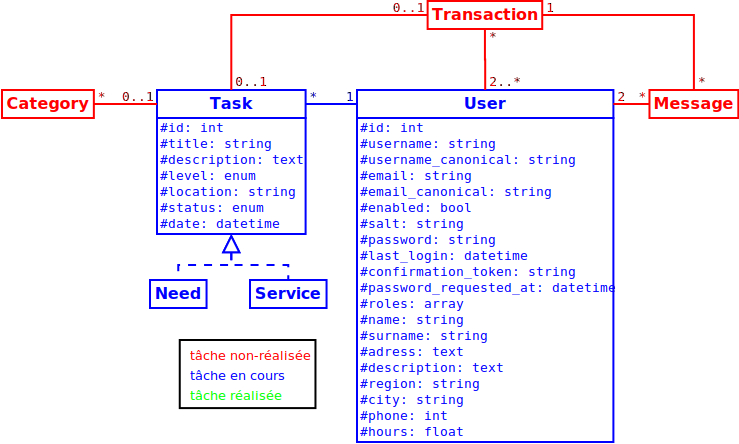
\includegraphics[width=\columnwidth]{uml}
				\caption{Diagramme de classes}
			\end{figure}
			\vspace*{\fill}

		\newpage
		\subsection{BPMN}

			\subsubsection{Utilisateurs}

				\vspace*{\fill}
				\begin{figure}[h]
					\centering
					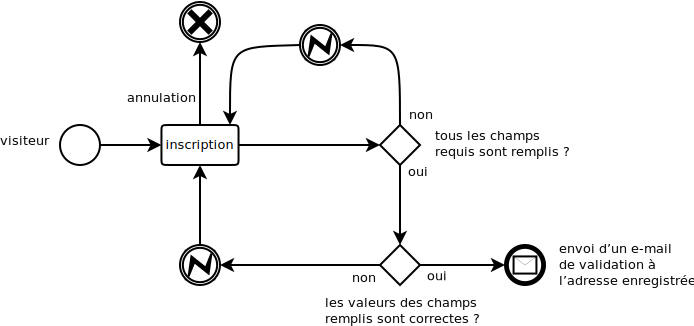
\includegraphics[width=\columnwidth]{bpmn-user-creation}
					\caption{Création d’un Utilisateur}
				\end{figure}
				\vspace*{\fill}

				\newpage
				\vspace*{\fill}
				\begin{figure}[h]
					\centering
					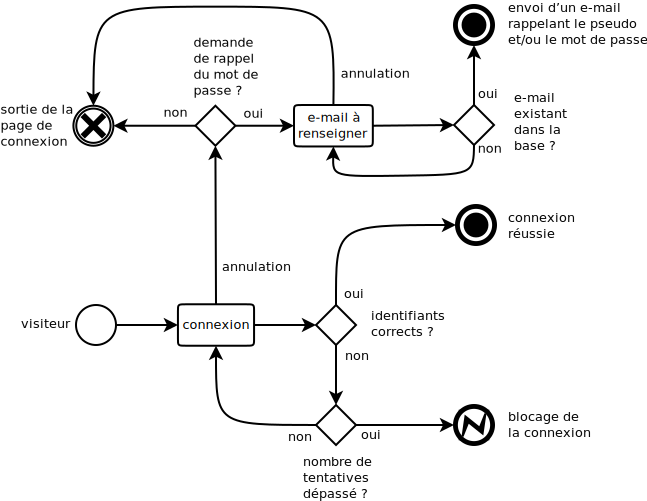
\includegraphics[width=\columnwidth]{bpmn-user-connection}
					\caption{Connexion d’un Utilisateur}
				\end{figure}
				\vspace*{\fill}

				\newpage
				\vspace*{\fill}
				\begin{figure}[h]
					\centering
					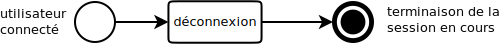
\includegraphics[width=\columnwidth]{bpmn-user-deconnection}
					\caption{Déconnexion d’un utilisateur}
				\end{figure}
				\vspace*{\fill}

				\newpage
				\vspace*{\fill}
				\begin{figure}[h]
					\centering
					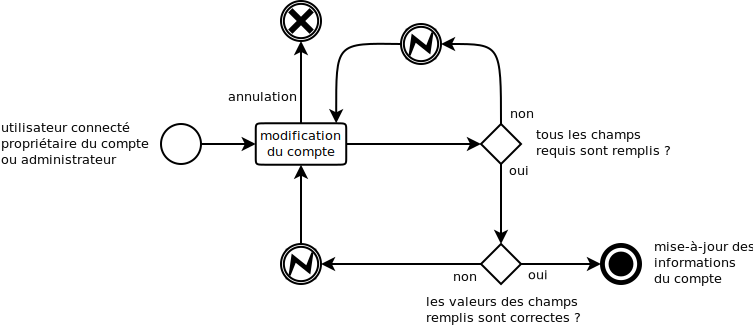
\includegraphics[width=\columnwidth]{bpmn-user-update}
					\caption{Mise-à-jour d’un Utilisateur}
				\end{figure}
				\vspace*{\fill}

				\newpage
				\vspace*{\fill}
				\begin{figure}[h]
					\centering
					
\includegraphics[width=\columnwidth]{bpmn-user-disabling}
					\caption{Désactivation d’un Utilisateur}
				\end{figure}
				\vspace*{\fill}

			\newpage
			\subsubsection{Tâches (Besoins ou Services)}

				\vspace*{\fill}
				\begin{figure}[h]
					\centering
					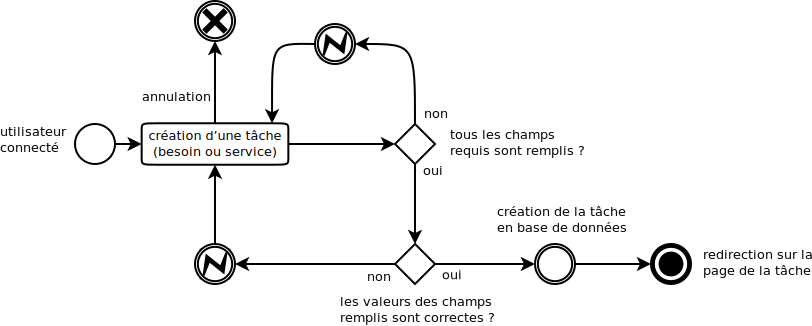
\includegraphics[width=\columnwidth]{bpmn-task-creation}
					\caption{Création d’une Tâche}
				\end{figure}
				\vspace*{\fill}

				\newpage
				\vspace*{\fill}
				\begin{figure}[h]
					\centering
					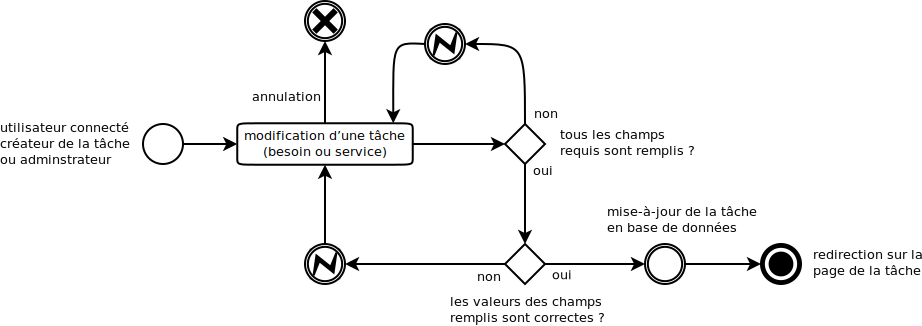
\includegraphics[width=\columnwidth]{bpmn-task-update}
					\caption{Mise-à-jour d’une Tâche}
				\end{figure}
				\vspace*{\fill}

				\newpage
				\vspace*{\fill}
				\begin{figure}[h]
					\centering
					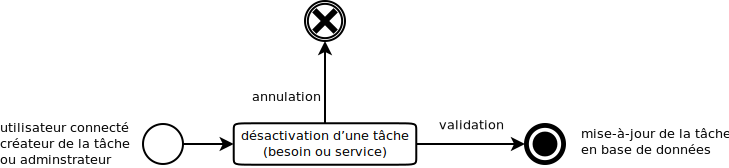
\includegraphics[width=\columnwidth]{bpmn-task-disabling}
					\caption{Désactivation d’une Tâche}
				\end{figure}
				\vspace*{\fill}

% Document ends here
\end{document}
